\documentclass{article}

\usepackage{fancyhdr}
\usepackage{extramarks}
\usepackage{amsmath}
\usepackage{graphicx}
\usepackage{pgfplotstable}

%
% Basic Document Settings
%

\topmargin=-0.45in
\evensidemargin=0in
\oddsidemargin=0in
\textwidth=6.5in
\textheight=9.0in
\headsep=0.25in

\linespread{1.1}

\pagestyle{fancy}
\lhead{\hmwkAuthorName}
\chead{\hmwkClass\ : \hmwkTitle}
\rhead{\firstxmark}
\lfoot{\lastxmark}
\cfoot{\thepage}

\renewcommand\headrulewidth{0.4pt}
\renewcommand\footrulewidth{0.4pt}

\setlength\parindent{0pt}

%
% Create Problem Sections
%

\newcommand{\enterProblemHeader}[1]{
    \nobreak\extramarks{}{Problem \arabic{#1} continued on next page\ldots}\nobreak{}
    \nobreak\extramarks{Problem \arabic{#1} (continued)}{Problem \arabic{#1} continued on next page\ldots}\nobreak{}
}

\newcommand{\exitProblemHeader}[1]{
    \nobreak\extramarks{Problem \arabic{#1} (continued)}{Problem \arabic{#1} continued on next page\ldots}\nobreak{}
    \stepcounter{#1}
    \nobreak\extramarks{Problem \arabic{#1}}{}\nobreak{}
}

\setcounter{secnumdepth}{0}
\newcounter{partCounter}
\newcounter{homeworkProblemCounter}
\setcounter{homeworkProblemCounter}{1}
\nobreak\extramarks{Problem \arabic{homeworkProblemCounter}}{}\nobreak{}

%
% Homework Problem Environment
%
% This environment takes an optional argument. When given, it will adjust the
% problem counter. This is useful for when the problems given for your
% assignment aren't sequential. See the last 3 problems of this template for an
% example.
%
\newenvironment{homeworkProblem}[1][-1]{
    \ifnum#1>0
        \setcounter{homeworkProblemCounter}{#1}
    \fi
    \section{Problem \arabic{homeworkProblemCounter}}
    \setcounter{partCounter}{1}
    \enterProblemHeader{homeworkProblemCounter}
}{
    \exitProblemHeader{homeworkProblemCounter}
}

%
% Homework Details
%   - Title
%   - Due date
%   - Class
%   - Section/Time
%   - Instructor
%   - Author
%

\newcommand{\hmwkTitle}{Homework\ \#2}
\newcommand{\hmwkDueDate}{January 30, 2015}
\newcommand{\hmwkClass}{PHYS 5243 - Solid State Physics}
\newcommand{\hmwkClassInstructor}{Professor Sheena Murphy}
\newcommand{\hmwkAuthorName}{Chase Brown}


\begin{document}




\begin{homeworkProblem}
    Explain the behavior of the specific heats for graphene, graphite, bundled SWCNTs and a single armchair (10,10) SWCNT using the Debye model and the acoustic phonon frequencies of these materials with the figure provided.
	

	\begin{description}
	\item[\textbf{Acoustic Mode Velocities:}] \hfill
		
		\begin{description}
		
			\item[Graphene:] \hfill
				\begin{enumerate}
					\item Longitudinal acoustic (LA): $ v = 24 \frac{km}{s} $
					\item In-plane transverse acoustic (iTA): $ v = 18 \frac{km}{s} $
					\item Out-of-plane transverse acoustic (oZA): $ \omega = \delta k^2, \delta \sim 6\times10^{-7} \frac{m^2}{s} $
				\end{enumerate}

			\item[(10,10) SWCNT:] \hfill
				\begin{enumerate}
					\item Transverse acoustic (TA): $ v = 9 \frac{km}{s} \rightarrow $ (Analogous to Combination of iTA and oTA in graphene) [two degenerate - perpendicular to SWCNT axis] 
					\item 'Twist' mode: $ v = 15 \frac{km}{s} \rightarrow $  (Torsion of SWCNT - analogous to iTA in graphene)
					\item Longitudinal acoustic (LA): $ v = 18 \frac{km}{s} \rightarrow $ (Directly analogous to LA mode in graphene) 
					\hfill
					\\
					All phonon modes show linear dispersion and there is no SWCNT phonon mode analogous to the ZA mode in graphene.
				\end{enumerate}


		\end{description}
	\end{description}

\hfill

	\centerline{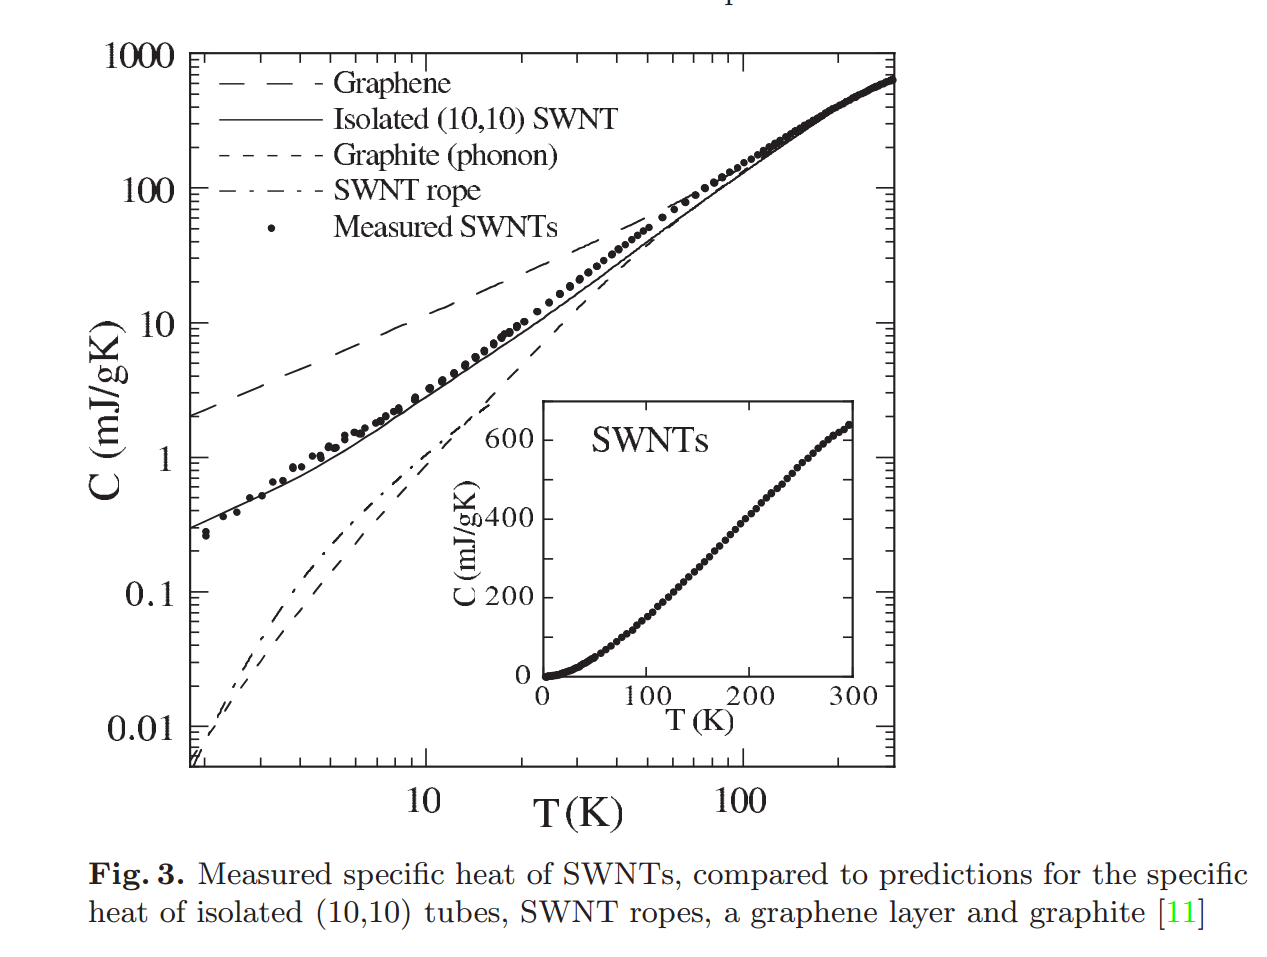
\includegraphics[scale=0.5]{CNTheatcapacity.png}}

\hfill

    \textbf{Solution} \hfill

		Graphene rigidity is increased as additional layers are added, which in turn increases the Debye frequency and Debye Temperature.  This increase in Debye Temperature decreases the heat capacity at a given low temperature.  
This effect is seen within the graph by the increase in heat capacity at low temperature from graphite to bundled nanotubes to a single SWCNT to graphene.
The graphite has the most interlayer interaction and rigidity, the bundled SWCNTs have some inter tube interaction and also added rigidity by the curvature, the individual SWCNT loses rigidity of the inter-tube coupling, and the graphene loses the rigidity of the curvature of the SWCNT.
\hfill
\\
We know that our momentum space dimensions will match the dimesions in real space of which the atoms are oscillating within.  Therefore, the minimum volume in k-space per mode is $ (\frac{2 \pi}{L})^{-D} $, while the number of allowed modes is:
\begin{equation*}
N \sim k^D L^D 
\end{equation*}

ALso, we know that

\begin{equation*}
N = \int_{0}^{\omega_D} d\omega D(\omega)
\end{equation*}
\begin{equation*}
E = \int_{0}^{\omega_D} d\omega D(\omega) \langle E_{\omega} \rangle
\end{equation*}
and 
\begin{equation*}
C = \frac{dE}{dT}
\end{equation*}
\begin{equation*}
C = C_{ph} + C_{e}
\end{equation*}
Where $D(\omega)$ is the phonon density of states.
Taking $\alpha$ to denote the dispersion relation $ \omega \propto k^{\alpha} $, we find that the phonon density of states (DOS or $\frac{dN}{d\omega}$) is dependent upon the dispersion relation and dimensionality of the system:

\begin{equation*}
\frac{dN}{d\omega} \propto k^{D-\alpha}
\end{equation*}


In addition, we can find how the heat capacity varies with temperature at temperatures much smaller than the Debye Temperature:

\begin{equation*}
	C_{ph} \propto T^{\frac{d}{\alpha}}
\end{equation*}

Which tells us that for graphene, 2 of our 3 modes have a $T^2$ dependence within this region ($\approx < 50K$), while one is linear in temperature with a much lower sound velocity.  Within this low temperature region, the out of plane (low velocity) modes are filed up very quickly and therefore it leads to a larger value for the heat capacity at low temperatures.
The metallic (10,10) armchair SWCNT has a cutting line which cuts directly through the K point within the graphene Brillouin zone, and therefore the electrons are very near the Fermi level and the electron contribution (while small compared to the phonon contribution) is greater in a metallic SWCNT than it would be for a semiconducting SWCNT (cutting line offset from the K point on the Dirac cone). Therefore, a semiconducting SWCNT would likely have a smaller value for the heat capacity at very low temperatures.  

\end{homeworkProblem}

\pagebreak




\begin{homeworkProblem}
	
	
	A Copper sample has dimensions of $ l=0.5 cm, w=2 cm,$ and $ t=2400$\AA  with a current of $I=400 mA$.  The following data are collected:

	\hfill

	\begin{tabular}{| c | c |}
		\hline

		\textbf{Magnetic Field (kG)} & \textbf{Voltage} \\
		\hline
		0 & 0.002 \\
		1.3 & 0.143 \\
		1.9 & 0.175 \\
		3.0 & 0.28 \\
		3.3 & 0.0315 \\
		4.5 & 0.0425 \\
		4.8 & 0.0425 \\
		5.9 & 0.056 \\
		6.3 & 0.0575 \\
		7.1 & 0.064 \\
		7.5 & 0.068 \\
		8.0 & 0.072 \\

		\hline
	\end{tabular}
	
	\begin{description}
		\item[a)] Calculate the hall coefficient.
		\item[b)] Make a determination of Avagadro's number from the Hall Coefficient.
	\end{description}

	\textbf{Solution} \hfill
	
	\textbf{a)} \hfill

		Plotting the Hall voltage versus the magnetic field given from the data reveals a slope related to the Hall coefficient:

		\hfill

		\centerline{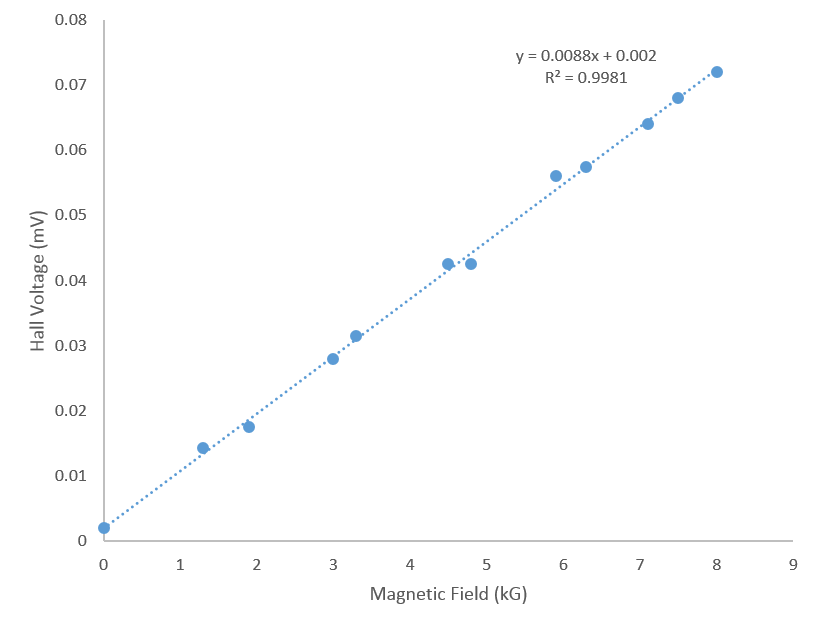
\includegraphics[scale=0.5]{VvsBPlot.png}}

		\hfill
		
		This slope is related to the Hall coefficient in the following way:

		\begin{equation*}
			\begin{aligned}
				V_H = R_H \frac{I}{t} B \\
				&
				\Rightarrow R_H \frac{I}{t} = 0.0088 \frac{mV}{kG} \\
				&
				\Rightarrow R_H = \frac{2400\AA}{400mA} (0.0088 \frac{mV}{kG}) \\
				&
				\Rightarrow R_H = 5.28 \times 10^{-11} \frac{m^3}{As} 
			\end{aligned}
		\end{equation*}

	\hfill

	\textbf{b)} \hfill
	
		Since $ R_H = \frac{-1}{ne} $ where n is the electron density of states, and e is the charge of the elecrton, the n should be proportional to the number of atoms per volume within the system as this metal is a good conductor.
		Thererfore:

		\begin{equation*}
			\begin{aligned}
				n = \frac{-1}{R_H e} = 1 \times 10^{29} \frac{1}{m^3} \\
				&
				N_A = \frac{n M_W}{\rho} \\
				&
				N_A = \frac{63.5 \frac{g}{mol} (1 \times 10^{29} \frac{1}{m^3}}{8960000 \frac{g}{m^3} } \\
				& 	
				\Rightarrow N_A = 7.087 \times 10^{23} \\
			\end{aligned}
		\end{equation*}

\end{homeworkProblem}

\pagebreak

\begin{homeworkProblem}

	\textbf{Simon - Solid State Basics:  (3.2) -Scattering Times}
		\begin{description}
			\item[a)] Calculate scattering times for Silver and Lithium using the data from the following table:
				
				\begin{tabular}{| c | c | c | c |}
					\hline
			
					 & $\rho (\Omega m) $ & $n (\frac{g}{cm^3})$ & $M_w (\frac{g}{mol})$ \\
					\hline
					Ag & $1.59 \times 10^8$ & 10.5 & 107.8 \\
					Li & $9.28 \times 10^8$ & 0.53 & 6.94 \\
					\hline
				\end{tabular}
			\item[b)] Calculate scattering time for Nitrogen using the following equation:
				\begin{equation*}
					\tau = \frac{1}{n \langle v \rangle \sigma}
				\end{equation*}
		\end{description}


	\textbf{Solution} 
	\hfill
	\textbf{a)}
	\hfill

		From equation 3.2 within Simon's text we find that:
			\begin{equation*}
				\begin{aligned}
				\sigma = \frac{e^2 \tau n}{m} = \frac{1}{\rho} \Rightarrow \tau = \frac{m}{\rho e^2 n} \\
				&
				\tau = \frac{m_e}{\rho e^2 n_e} \\
				&
				n_e = \frac{\rho_{Li} N_A e}{M_{W,Li}} = \frac{rho_{Li} F}{M_{W,Li}} 
				\end{aligned}
			\end{equation*}
		Where $F$ is Faraday's constant, $\tau$ is the scattering time, $\sigma$ is the conductivity, $\rho$ is the resistivity, $\rho_{Li}$ is the density of Lithium, $M_{W,Li}$ is the molecular wieght of Lithium, $n_e$ is the electron density, and $m_e$ is the mass of the electron. 

		We then find that:
			\begin{equation*}
				\begin{aligned}
				\tau_{Li} = \frac{m_e M_{W,Li}}{\rho e^2 \rho_{Li} F} \\
				&
				\tau_{Li} = \frac{(9.10938 \times 10^{-31} kg) (6.94 \frac{g}{mol})}{(9.28 \times 10^8 \Omega m)(1.602 \times 10^{-19} C)^2 (0.53 \frac{g}{cm^3})(9.648 \times 10^4 \frac{C}{mol})} \\
				&
				\tau_{Li} = 8.316 \times 10^{-31} s \\
				&
				\tau_{Ag} = 3.813 \times 10^{-30} s
				\end{aligned}
			\end{equation*}
		
	\textbf{b)}
	\hfill
		
		Using the equation given:
			\begin{equation*}
				\begin{aligned}
					\tau = \frac{1}{n \langle v \rangle \sigma} \\
					&
					\sigma = \pi d^2 \\
					&
					\langle v \rangle = \sqrt{\frac{8 k_B T}{\pi m}} \\
					& 
					\Rightarrow \tau = \frac{1}{n \pi d^2} \sqrt{\frac{\pi m}{8 k_B T}} \\
					&
					\rho = 0.001251 \frac{g}{mol} & (T = 298K) \\
					&
					n = \frac{\rho }{M_W amu} = \frac{0.001251 \frac{g}{mol}}{28 (1.66 \times 10^{-27} kg)} = 2.69 \times 10^{28} \frac{1}{m^3 kg} \\
					& 
					\Rightarrow \tau_{N_2} \approx 2 \times 10^{-10} s
				\end{aligned}
			\end{equation*}
		
			
\end{homeworkProblem}

\pagebreak

\begin{homeworkProblem}

	\textbf{Simon - Solid State Basics:  (3.3) - Ionic Conduction and Two Carrier Types} 
	\hfill

	Mixed ion conductors with electrons described by $n_e$ and $\tau_e$ for density and scattering time, and ions described simlarly with $n_i$ and $\tau_i$ calculate:
		\begin{description}
			\item[a)] Electrical Resistivity
			\item[b)] Thermal Conductivity
		\end{description}


	\textbf{Solution} 
	\hfill

	\textbf{a) Electrical Resistivity}
	\hfill
	
	\begin{equation*}
		\begin{aligned}
			\frac{1}{\rho} = \frac{n e^2 \tau}{m} \\
			&
			let \rho = \rho_i + \rho_e \\
			&
			\Rightarrow \rho = \frac{1}{\sigma_i} + \frac{1}{\sigma_e} \\
			& 
			\rho = \frac{m_e}{e^2 \tau_e n_e} + \frac{m_i}{e^2 \tau_i n_i}
		\end{aligned}
	\end{equation*}

	\hfill

\textbf{b) Thermal Conductivity}
	\hfill
	
	\begin{equation*}
		\begin{aligned}
			k = k_e + k_i \\
			&
			k = \frac{4 n \tau {k_B}^2 T}{\pi m} \\
			&
			\Rightarrow k = \frac{4 {k_B}^2 T}{\pi} (\frac{n_e \tau_e}{m_e} + \frac{n_i \tau_i}{m_i})
		\end{aligned}
	\end{equation*}

\end{homeworkProblem}

\end{document}